%%%%%%%%%%%%%%%%%%%%%%%%%%%%%%%%%%%%%%%%%
% Engineering Calculation Paper
% LaTeX Template
% Version 1.0 (20/1/13)
%
% This template has been downloaded from:
% http://www.LaTeXTemplates.com
%
% Original author:void fusion(int T[], int inicial, int final, int U[], int V[]){
% Dmitry Volynkin (dim_voly@yahoo.com.au)
%
% License:
% CC BY-NC-SA 3.0 (http://creativecommons.org/licenses/by-nc-sa/3.0/)
%
%%%%%%%%%%%%%%%%%%%%%%%%%%%%%%%%%%%%%%%%%

%----------------------------------------------------------------------------------------
%	PACKAGES AND OTHER DOCUMENT CONFIGURATIONS
%----------------------------------------------------------------------------------------

\documentclass[11pt,a4paper]{article} % Use A4 paper with a 12pt font size - different paper sizes will require manual recalculation of page margins and border positions

\usepackage[utf8]{inputenc}
\usepackage[spanish]{babel}
\usepackage{color}
\definecolor{gray97}{gray}{.97}
\definecolor{gray75}{gray}{.75}
\definecolor{gray45}{gray}{.45}
\usepackage{graphicx}
\usepackage{float}
\usepackage{listings}
\lstset{language=C++,
	frame=Ltb,
	framerule=0pt,
	aboveskip=.5cm,
	framextopmargin=3pt,
	framexbottommargin=3pt,
	framexleftmargin=0.2cm,
	framexrightmargin=0cm,
	framesep=0pt,
	rulesep=1.4pt,
	backgroundcolor=\color{gray97},
	rulesepcolor=\color{gray45},
	%
	stringstyle=\color{red!80!black}\ttfamily,
	showstringspaces = false,
	basicstyle=\ttfamily,
	commentstyle=\color{green!50!black}\ttfamily,
	keywordstyle=\color{blue}\ttfamily,
	morecomment=[l][\color{magenta}]{\#},
	%
	numbers=left,
	numbersep=10pt,
	numberstyle=\tiny,
	numberfirstline = false,
	breaklines=true,
	postbreak=\mbox{\textcolor{red}{$\hookrightarrow$}},
	xleftmargin=0.7cm,
	xrightmargin=0.3cm,
	tabsize=4,
}

% minimizar fragmentado de listados
\lstnewenvironment{listing}[1][]
{\lstset{#1}\pagebreak[0]}{\pagebreak[0]}

\lstdefinestyle{consola}
{basicstyle=\scriptsize\bf\ttfamily,
	backgroundcolor=\color{gray75},
}

\lstdefinestyle{C++}
{language=C++,
}


\usepackage{marginnote} % Required for margin notes
\usepackage{wallpaper} % Required to set each page to have a background
\usepackage{lastpage} % Required to print the total number of pages
\usepackage[left=1.3cm,right=4.6cm,top=2cm,bottom=4.0cm,marginparwidth=3.4cm]{geometry} % Adjust page margins
\usepackage{amsmath} % Required for equation customization
\usepackage{amssymb} % Required to include mathematical symbols
\usepackage{xcolor} % Required to specify colors by name
\usepackage{fancyhdr} % Required to customize headers
\setlength{\headheight}{80pt} % Increase the size of the header to accommodate meta-information
\pagestyle{fancy}\fancyhf{} % Use the custom header specified below
\renewcommand{\headrulewidth}{0pt} % Remove the default horizontal rule under the header

\setlength{\parindent}{0cm} % Remove paragraph indentation
\newcommand{\tab}{\hspace*{2em}} % Defines a new command for some horizontal space

\newcommand\BackgroundStructure{ % Command to specify the background of each page
\setlength{\unitlength}{1mm} % Set the unit length to millimeters

\setlength\fboxsep{0mm} % Adjusts the distance between the frameboxes and the borderlines
\setlength\fboxrule{0.5mm} % Increase the thickness of the border line
\put(10, 10){\fcolorbox{black}{blue!10}{\framebox(155,247){}}} % Main content box
\put(165, 10){\fcolorbox{black}{blue!10}{\framebox(37,247){}}} % Margin box
\put(10, 261){\fcolorbox{black}{white!10}{\framebox(192, 27){}}} % Header box
\put(145, 270){
\includegraphics[height=15mm,keepaspectratio]{../logo.png}} % Logo box - maximum height/width: 
}

%----------------------------------------------------------------------------------------
%	HEADER INFORMATION
%----------------------------------------------------------------------------------------

\fancyhead[L]{\begin{tabular}{l r | l r} % The header is a table with 4 columns
		\textbf{ALGORÍTMICA} &  & \textbf{Adrián Carmona Lupiáñez} \\ % Project name and page count
		\textbf{Práctica} & 3 & \textbf{Ignacio Sánchez Herrera}  \\ % Version and reviewed date
		&  & \textbf{Jacobo Casado de Gracia} \\
		\textbf{Página} & \thepage/\pageref{LastPage} & \textbf{Jesús José Mª Maldonado Arroyo} \\
		& & \textbf{Juan Miguel Hernández Gómez} \\
\end{tabular}}

%----------------------------------------------------------------------------------------

\begin{document}

\AddToShipoutPicture{\BackgroundStructure} % Set the background of each page to that specified above in the header information section

%----------------------------------------------------------------------------------------
%	DOCUMENT CONTENT
%----------------------------------------------------------------------------------------

En esta práctica vamos a analizar el uso de los algoritmos “voraces” o “greedy”, algoritmos que seleccionan en cada momento lo mejor de entre un conjunto de candidatos, sin tener en cuenta lo ya hecho, para obtener una solución “rápida” al problema.\\

Vamos a tener dos problemas a los cuales vamos a aplicar esta manera de resolverlos y mediremos su eficiencia teórica.\\

Una vez diseñado el algoritmo, veremos los resultados de la ejecución y los compararemos con los resultados “óptimos”, generados tras resolver el problema de la menor manera posible.\\

Recordemos que los algoritmos greedy no aseguran generar soluciones optimales siempre; esta desventaja es una ventaja en problemas en los que es muy difícil alcanzar la solución óptima, apliquemos el algoritmo que apliquemos, como el problema que se propone a continuación. No obstante, veremos que los resultados, a pesar de no ser los óptimos, son bastante eficientes, así como el tiempo de ejecución del algoritmo.\\


\section{Problema común (Viajante de comercio)}

Como hemos comentado anteriormente, aplicar un algoritmo que nos dé el resultado más óptimo para este problema es bastante complicado y su tiempo de ejecución se incrementaría bastante.\\

Es por eso por lo que el enfoque Greedy es una manera eficiente de solucionar este problema, generando un resultado que no es el óptimo pero se acerca a ello.\\

El problema se resume en encontrar un circuito hamiltoniano para una serie de puntos, en este caso ciudades, de manera que se recorran todas ellas sin volver a pasar por ninguna, de manera que la distancia total entre estas ciudades, es decir, del circuito, sea la mínima (y así minimizamos el recorrido).\\

\subsection{Algoritmo basado en cercanía}

En primer lugar, hemos desarrollado una estrategia basada en encontrar el “vecino más cercano”: tomamos una ciudad inicial inicial de manera arbitraria, y buscamos en el vector de ciudades que no se han visitado la ciudad más cercana a esta. Una vez encontrada, se procede a hacer un borrado lógico de la ciudad en el vector, y se procede a encontrar la ciudad más cercana a esta última visitada.\\

El procedimiento se repite hasta que todas las ciudades se hayan visitado, obteniendo el camino.\\

Hemos creado también una clase matriz que hemos usado de forma auxiliar para simplificar la parte del código del algoritmo que se detalla a continuación.\\

\subsubsection{Código del programa}
\begin{lstlisting}[style=C++]
#include <iostream>
#include <fstream>
#include <string>
#include <vector>
#include <utility>
#include <cmath>
#include <limits>
#include "matriz.h"

using namespace std;
const double INF = numeric_limits<double>::max();


/*  FUNCION
*  Esta funcion recibe como parametros un vector, que son las distintas distancias
* a las distintas ciudades desde una misma ciudad y el vector candidatos para comprobar 
* si ya se han visitado las respectivas ciudades.
* 
* La funcion encuentra el menor elemento del vector v y devuelve la posicion dentro
* del vector de dicho elemento.
*/
int BuscaMenor(vector<double> v, vector<int> & candidatos){
	int menor;
	double minimo = INF;
	for(int i = 0;i< v.size(); ++i){
		if( v[i] < minimo && candidatos[i] !=-1){
			minimo = v[i];
			menor = i;
		}
	}
	return(menor);
}


int main(int argc, char **argv){

	ifstream input_file(argv[1]);
	string line;
	int dimension;

	int ciudad;
	double coor_x, coor_y;

	vector<pair<double, double> > v;
	pair<double, double> p;
	
	//Movemos el offset a la linea en la que se dice la dimension del grafo
	for(int i=0; i<3; ++i){
		getline(input_file, line);
	}
	
	getline(input_file, line);
	line.erase(0, 11);
	dimension = atoi(line.c_str());
	
	//Reservamos espacio para el grafo
	matriz <double> m(dimension, dimension, INF);
	
	//Movemos el offset al comienzo de los datos
	for(int i=0; i<3; ++i){
		getline(input_file, line);
	}
	
	//Tomamos los datos
	for (int i=0; i<dimension; ++i){
		input_file >> ciudad;
		input_file >> coor_x;
		input_file >> coor_y;
		p.first = coor_x;
		p.second = coor_y;
		v.push_back(p);
	}
	
	//Calculamos las distancias y las metemos en la matriz que representa
	//el grafo
	for(int i=0; i<dimension; ++i){
		for (int j=i+1; j<dimension; ++j){
			m[i][j]=sqrt(pow(v[j].first - v[i].first, 2) + pow(v[j].second - v[i].second, 2));
			m[j][i]=m[i][j];
		}
	}
	
	//Algoritmo basado en cercanias. La idea es ir a la ciudad mas cercana
	//sin formar un ciclo. Exceptuando la ultima.
	
	//Declaramos los vectores que albergaran los conjuntos Candidato y Solucion
	vector<int> solucion;
	vector<int> candidatos;
	
	// Inicializamos el conjunto de candidatos, el rango sera [0,15]. 
	for(int i = 0; i<dimension;++i){
		candidatos.push_back(i);
	}
	
	// Abergamos la primera ciudad en el conjunto solucion.
	int i = 0;
	solucion.push_back(0);
	candidatos[0] = -1;
	
	// variable donde guardaremos el indice, es decir, la ciudad a donde nos dirigimos.
	int menor;
	
	/*CUERPO DEL ALGORITMO:
	* La idea es encontrar la ciudad mas cercana haciendo uso de la matriz de
	* distancias. Una vez encontrada la ciudad (indice) al que nos dirigimos,
	* la posicion candidatos[indice] lo hacemos -1 para mostrar que esa ciudad
	* ya la hemos visitado y introducimos el indice en el vector de soluciones.
	* 
	* Para concluir, asignamos el valor del indice a la variable i para empezar
	* de nuevo todo el proceso
	*/
	while(solucion.size()< dimension   ){
		vector <double> c;
		m.get_Fila(i,c);
		menor =BuscaMenor(c, candidatos);
		solucion.push_back(menor);
		candidatos[menor] = -1;
		i = menor;
	}
	
	// Imprimimos el vector solucion teniendo en cuenta que para la implementacion
	// La ciudad numero 1 ha sido el indice numero 0, por lo tanto tenemos que sumar
	// 1 a los valores del vector solucion.
	
	for(int i = 0; i< solucion.size();i++){
		cout << solucion [i]  + 1<< " --> ";
	}
	// Aniadimos la ciudad inicial para indicar que completamos un ciclo.
	cout << " 1 " << " FIN.";
	
	
	// Volcamos la salida a un fichero para su visualizacion con la ayuda de 
	// GNUPLOT.
	
	ofstream ficherosalida("data/ulysses_camino.txt");
	for (int i = 0; i < dimension; ++i){
		int c = solucion[i];
		ficherosalida << c+1 << " " << v[c].first << " " << v[c].second << endl;
	}
	
	
	//FIN.
	return (0);
}
\end{lstlisting}

\subsubsection{Pseudocódigo}
El algoritmo por cercanía en pseudocódigo es el siguiente:
\begin{lstlisting}
N = |V|
S = {primera ciudad de V}
Repetir
	U = Buscar ciudad del conjunto V mas cercana a la ultima ciudad insertada en S
	Eliminar U de V
	Insertar U en S
Hasta que |S| = N
Insertar de nuevo en S la primera ciudad que habiamos insertado al principio
Devolver S
\end{lstlisting}

\subsubsection{Visualización}
\begin{figure}[H]
	\centering
	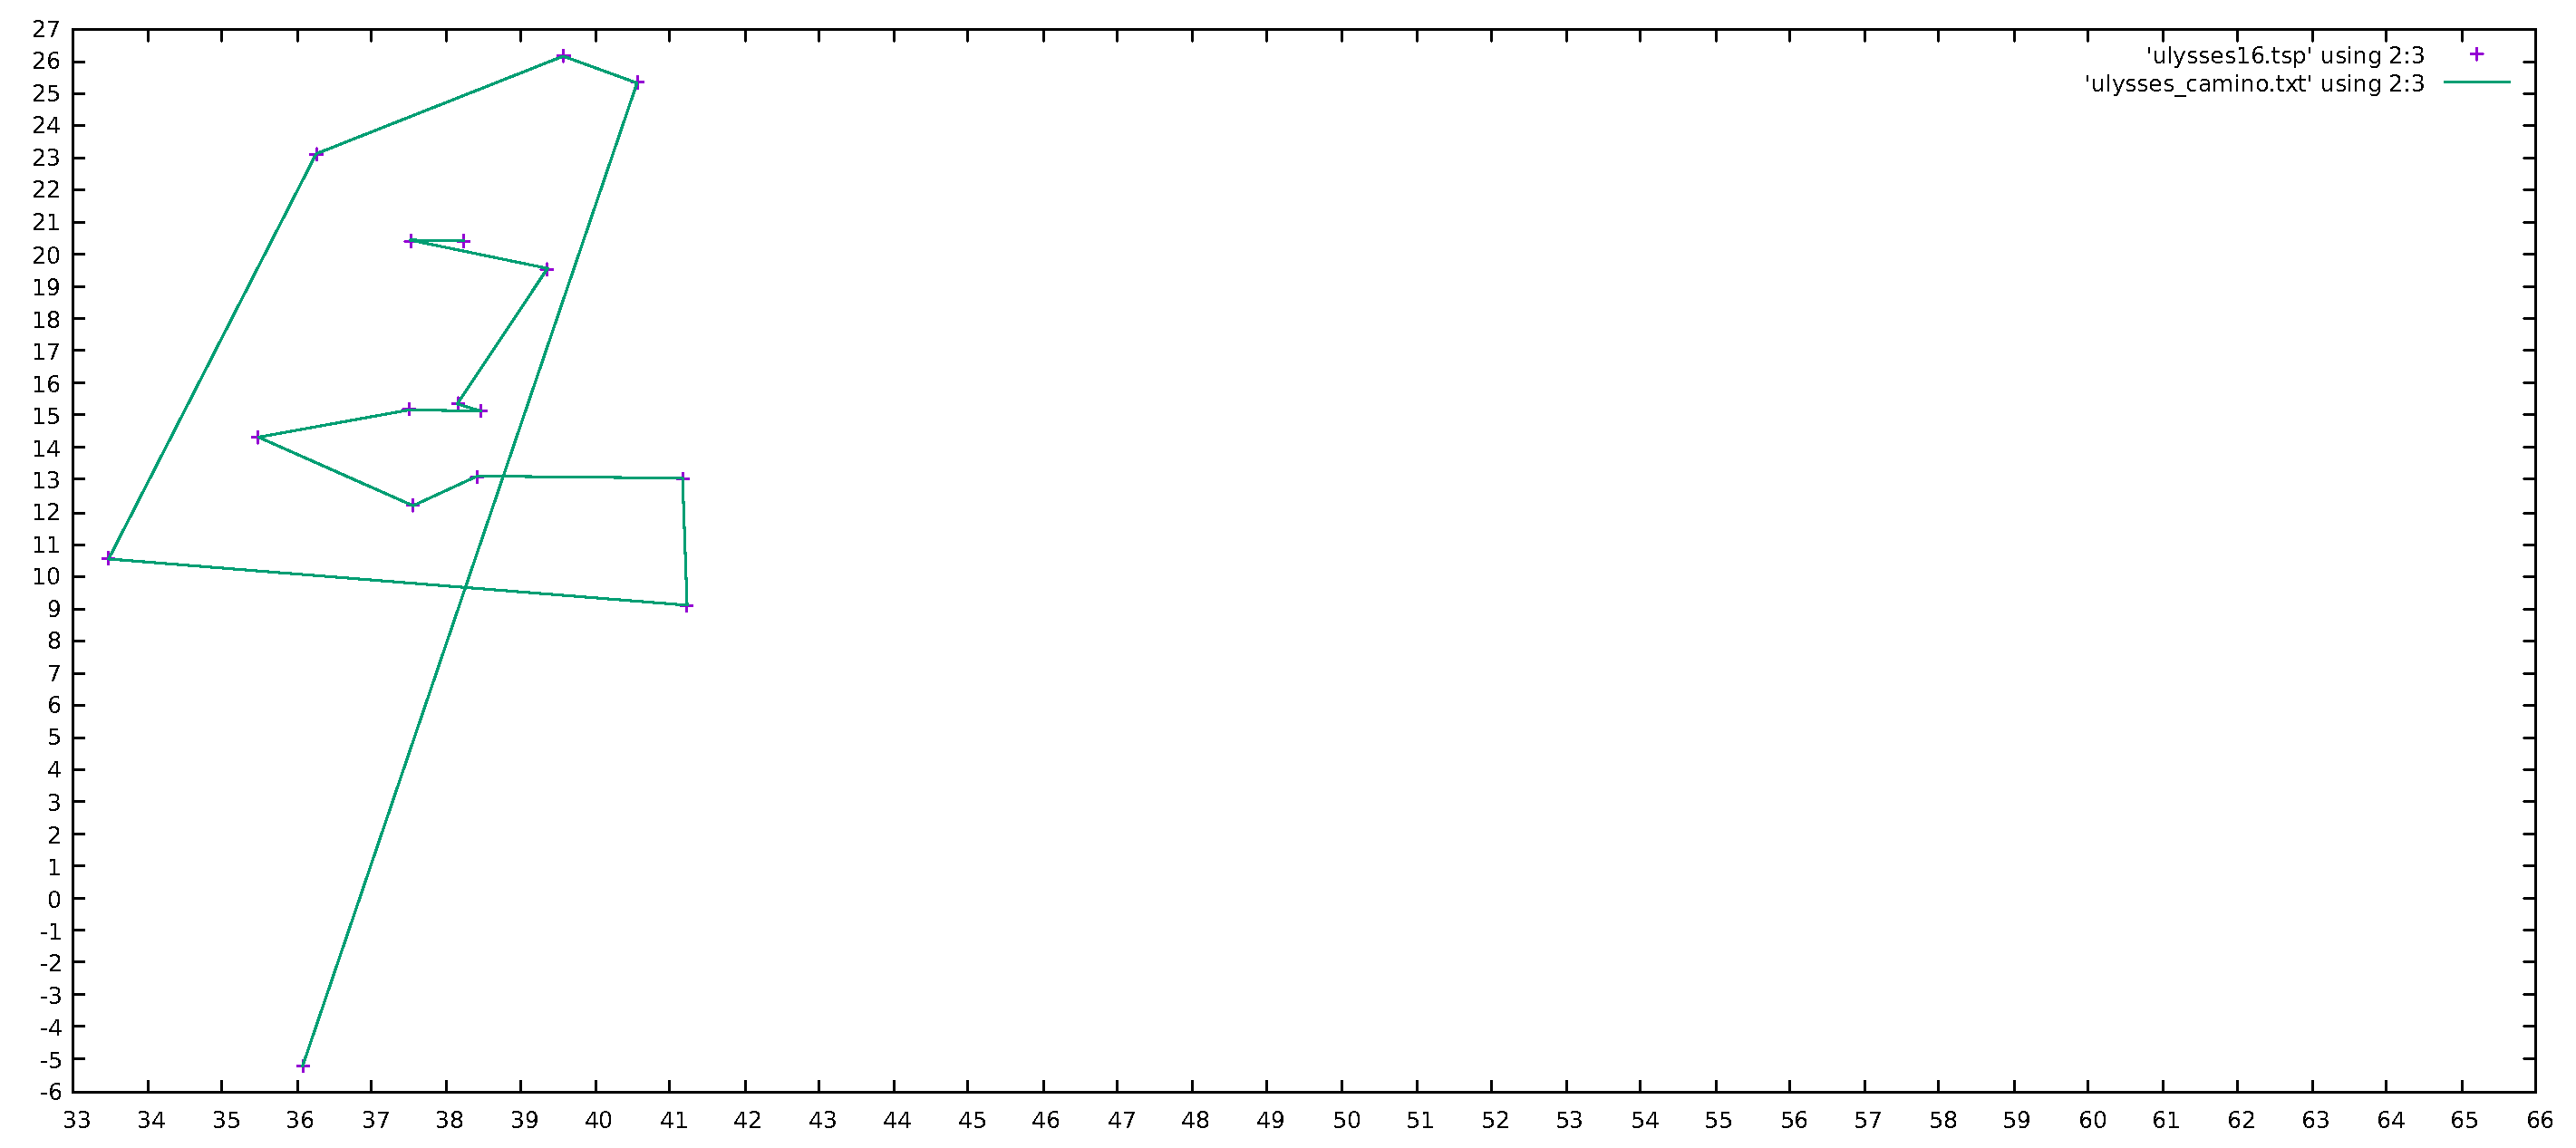
\includegraphics[width=13cm]{data/graphics/cercania/cercania.pdf}
\end{figure}

\subsubsection{Eficiencia teórica}
La eficiencia teórica O(n) depende del número de ciudades que hay. Tomamos, por tanto, $TAM = dimension = n$.\\

La eficiencia del algoritmo, en el peor de los casos, es 
$$T(n) = \sum_{i=1}^{n}\sum_{j=1}^{n}$$
$$T(n) = n*n$$
$$T(n) \in O(n^2)$$\\

Esto es debido a que la función $BuscaMenor$ es de tiempo $n$, y se ejecuta también $n$ veces en el bucle $while$ de la línea 112.



\newpage
\subsection{Algoritmo basado en inserción}
Este algoritmo greedy para resolver el problema del viajante de comercio consiste en partir de un circuito inicial. En nuestro caso las ciudades elegidas para el circuito inicial son la más al Este, la más al Oeste y la más al Norte. Una vez escogido el recorrido inicial comienza el algoritmo. Nuestro algoritmo de inserción se basa en insertar en cada iteración la ciudad que menos aumenta el tamaño de este.

\subsubsection{Código del programa}
\begin{lstlisting}[style=C++]
#include <iostream>
#include <fstream>
#include <string>
#include <vector>
#include <utility>
#include <cmath>
#include <limits>
#include "matriz.h"

using namespace std;


/**
Este programa busca un ciclo que recorra todas las ciudades de un mapa mediante un algoritmo de tipo greedy. En esta version del algoritmo, dado un recorrido inicial que contiene tres nodos en cada paso se busca el nodo mas cercano al conjunto solucion que se encuentre en el conjunto de candidatos. El nodo mas cercano es insertado en la posicion del vector que menos aumente el recorrido.
*/
int main(int argc, char **argv){
	const double INF = numeric_limits<double>::max();
	
	if(argc < 2){
		cout << "ERROR. Faltan argumentos [archivo de datos]" << endl;
		exit(-1);
	}
	
	ifstream input_file(argv[1]);
	string line;
	int num_ciudades;
	
	int ciudad;
	double coor_x, coor_y;
	
	vector<pair<double, double> > v_coordenadas;
	pair<double, double> coordenadas;
	
	vector<int> candidatos;
	vector<int> solucion;
	
	//Movemos el offset a la linea en la que se dice la dimension del grafo
	for(int i=0; i<3; ++i){
		getline(input_file, line);
	}
	
	getline(input_file, line);
	line.erase(0, 11);
	num_ciudades = atoi(line.c_str());
	
	//Reservamos espacio para el grafo
	matriz <double> distancias(num_ciudades, num_ciudades, 0);
	
	//Movemos el offset al comienzo de los datos
	for(int i=0; i<3; ++i){
		getline(input_file, line);
	}
	
	//Tomamos los datos
	for (int i=0; i<num_ciudades; ++i){
		input_file >> ciudad;
		input_file >> coor_x;
		input_file >> coor_y;
		coordenadas.first = coor_x;
		coordenadas.second = coor_y;
		v_coordenadas.push_back(coordenadas);
	}
	
	//Calculamos las distancias y las metemos en la matriz que representa
	//el grafo
	for(int i=0; i<num_ciudades; ++i){
		for (int j=i+1; j<num_ciudades; ++j){
			distancias[i][j]=sqrt(pow(v_coordenadas[j].first - v_coordenadas[i].first, 2) +
			pow(v_coordenadas[j].second - v_coordenadas[i].second, 2));
			distancias[j][i]=distancias[i][j];
		}
	}
	
	distancias.draw();
	
	//Generamos vector de candidatos
	for(int i=0; i<num_ciudades; ++i)
		candidatos.push_back(i);
	
	//Elegimos el recorrido inicial
	int E = 0, O = 0, N = 0;
	double mas_al_E = v_coordenadas[0].first;
	double mas_al_O = v_coordenadas[0].first; 
	double mas_al_N = v_coordenadas[0].second;
	
	for(int i=1; i<num_ciudades; ++i){
		if(v_coordenadas[i].second > mas_al_N){
			mas_al_N = v_coordenadas[i].second;
			N = i;
		}
		if(v_coordenadas[i].first > mas_al_E){
			mas_al_E = v_coordenadas[i].first;
			E = i;
		}
		if(v_coordenadas[i].first < mas_al_O){
			mas_al_O = v_coordenadas[i].first;
			O = i;
		}
	}
	
	solucion.push_back(O); candidatos[O] = -1;
	solucion.push_back(N); candidatos[N] = -1;
	solucion.push_back(E); candidatos[E] = -1;
	
	int tam_solucion = solucion.size(); //Tamanio del conjunto solucion
	
	//Comienzo del algoritmo
	vector<int>::iterator sol_it, cand_it;  //Iteradores de los vectores de candidatos y solucion
	vector<int>::iterator ciudad_origen_it; //Iterador que almacenara la posicion de la ciudad del
	//conjunto solucion, que tiene mas cerca a una ciudad
	//del conjuno candidatos    
	
	while(tam_solucion < num_ciudades){ //Mientras que no hayamos recorrido todas las ciudades
		//Buscamos la ciudad mas cercana al conjunto solucion
		int ciudad_mas_cercana = 0;
		double distancia_mas_cercana = INF;
		
		for(sol_it=solucion.begin(); sol_it!=solucion.end(); ++sol_it){
			for (cand_it=candidatos.begin(); cand_it!=candidatos.end(); ++cand_it){
				if ((distancias[*sol_it][*cand_it] < distancia_mas_cercana) && (*cand_it != -1)){
					ciudad_origen_it = sol_it;
					ciudad_mas_cercana = *cand_it;
					distancia_mas_cercana = distancias[*sol_it][*cand_it];
				}
			}
		}
		
		//Una vez encontrada vemos en que posicion del conjunto solucion insertarla para minimizar el trayecto
		vector<int>::iterator ciudad_siguiente_it = ciudad_origen_it;
		vector<int>::iterator ciudad_anterior_it = ciudad_origen_it;
		vector<int>::iterator final_it = solucion.end();
		final_it--;
		
		//Puesto que el recorrido es un ciclo (cerrado) hay que contemplar el caso de que la
		//ciudad a insertar sea adyacente al primer o ultimo elemento del conjunto solucion
		if(ciudad_origen_it == solucion.begin()){
			++ciudad_siguiente_it;
			ciudad_anterior_it = final_it;
		}
		else if(ciudad_origen_it == final_it){
			ciudad_siguiente_it = solucion.begin();
			--ciudad_anterior_it;
		}
		else{
			++ciudad_siguiente_it;
			--ciudad_anterior_it;
		}
		
		
		if(distancias[ciudad_mas_cercana][*ciudad_anterior_it] < distancias[ciudad_mas_cercana][*ciudad_siguiente_it]){
			solucion.insert(ciudad_origen_it, ciudad_mas_cercana);
		}
		else{
			solucion.insert(ciudad_siguiente_it, ciudad_mas_cercana);
		}
		
		candidatos[ciudad_mas_cercana] = -1;
		tam_solucion++;
	}
	
	//Insertamos de nuevo el primer elemento del conjunto solucion
	// ya que es un caamino cerrado
	solucion.push_back(*solucion.begin());
	
	//Mostramos la solucion
	cout << "Solucion: " << endl;
	
	for(int i=0; i<tam_solucion; ++i){
		cout << solucion[i]+1 << " ";
	}
	cout << endl;
	
	//Calculo de la distancia total recorrida
	double distancia_recorrida = 0.00;
	for(int i=0; i<tam_solucion-1; ++i){
		distancia_recorrida += distancias[i][i+1];
	}
	
	cout << "Distancia total recorrida: " << distancia_recorrida << endl;
	
	//Salida de la solucion a fichero
	ofstream output_file("data/ulysses16_insercion.txt");
	for(int i=0; i<num_ciudades; ++i){
		int c = solucion[i];
		output_file << c+1 << " " << v_coordenadas[c].first << " " << v_coordenadas[c].second << endl;
	}
	
	return (0);
}
\end{lstlisting}

\subsubsection{Pseudocódigo}
El algoritmo por inserción en pseudocódigo es el siguiente:
\begin{lstlisting}
N = |V|
S = {ciudad mas al Norte, 
	ciudad mas al Este, 
	ciudad mas al Oeste}
Repetir
	U = Buscar ciudad del conjunto V que menos aumenta la distancia de S
	Eliminar U de V
	Insertar U en S
Hasta que |S| = N
Devolver S
\end{lstlisting}

\subsubsection{Visualización}
Empezamos seleccionando 3 ciudades distanciadas.
\begin{figure}[H]
	\centering
	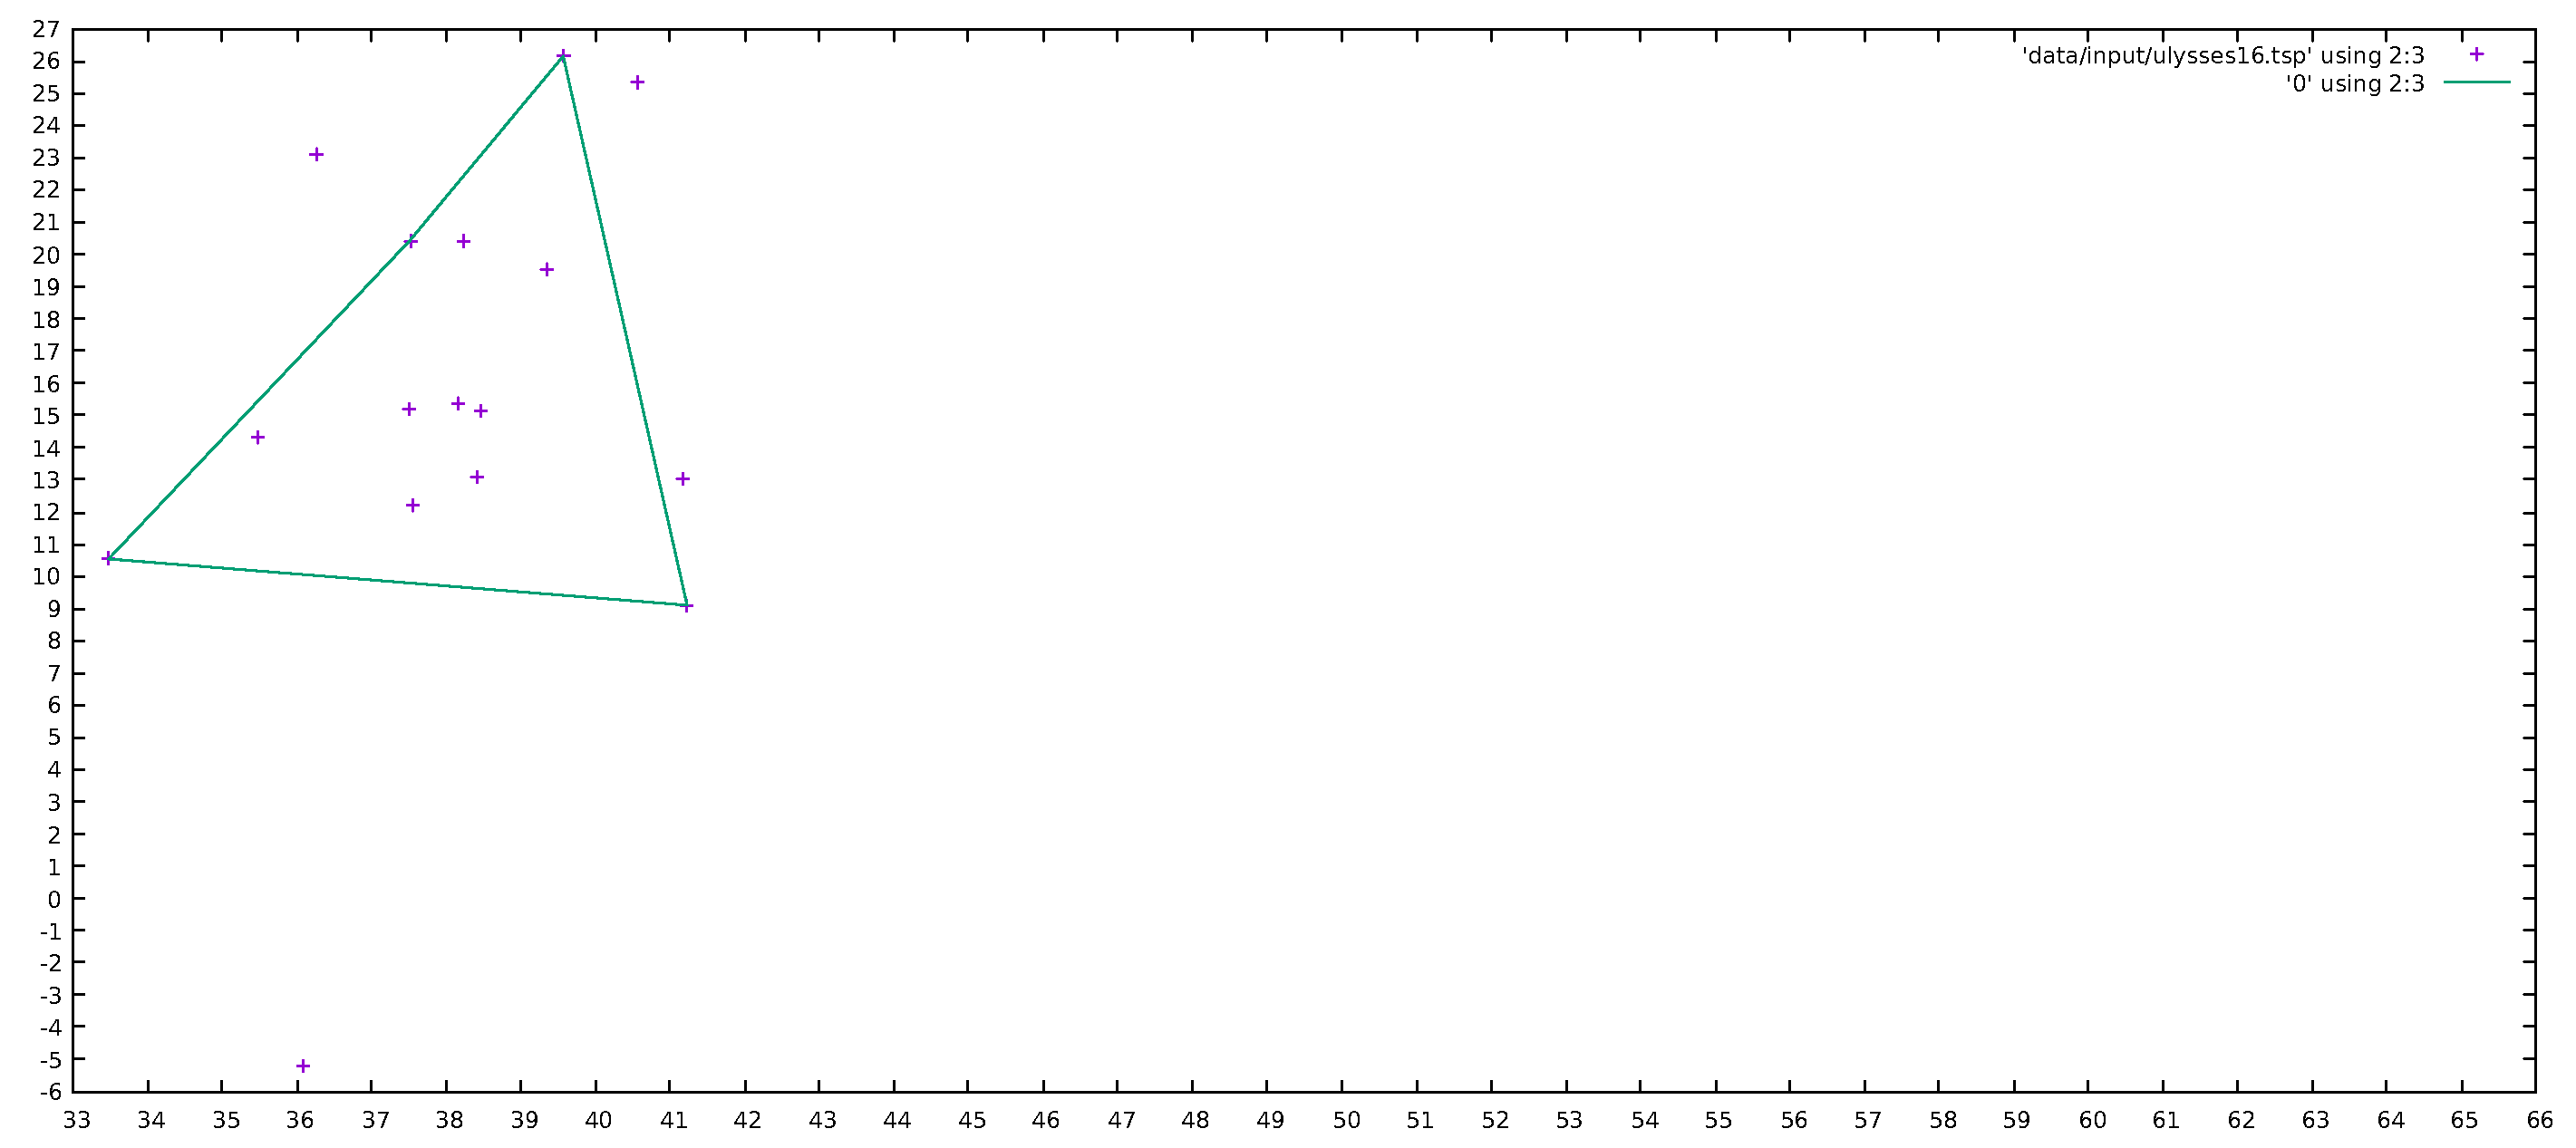
\includegraphics[width=13cm]{data/graphics/insercion/insercion_1.pdf}
\end{figure}
\vspace{0,7cm}

Continuamos añadiendo aquella ciudad que aumente en menor medida el recorrido total.
\begin{figure}[H]
	\centering
	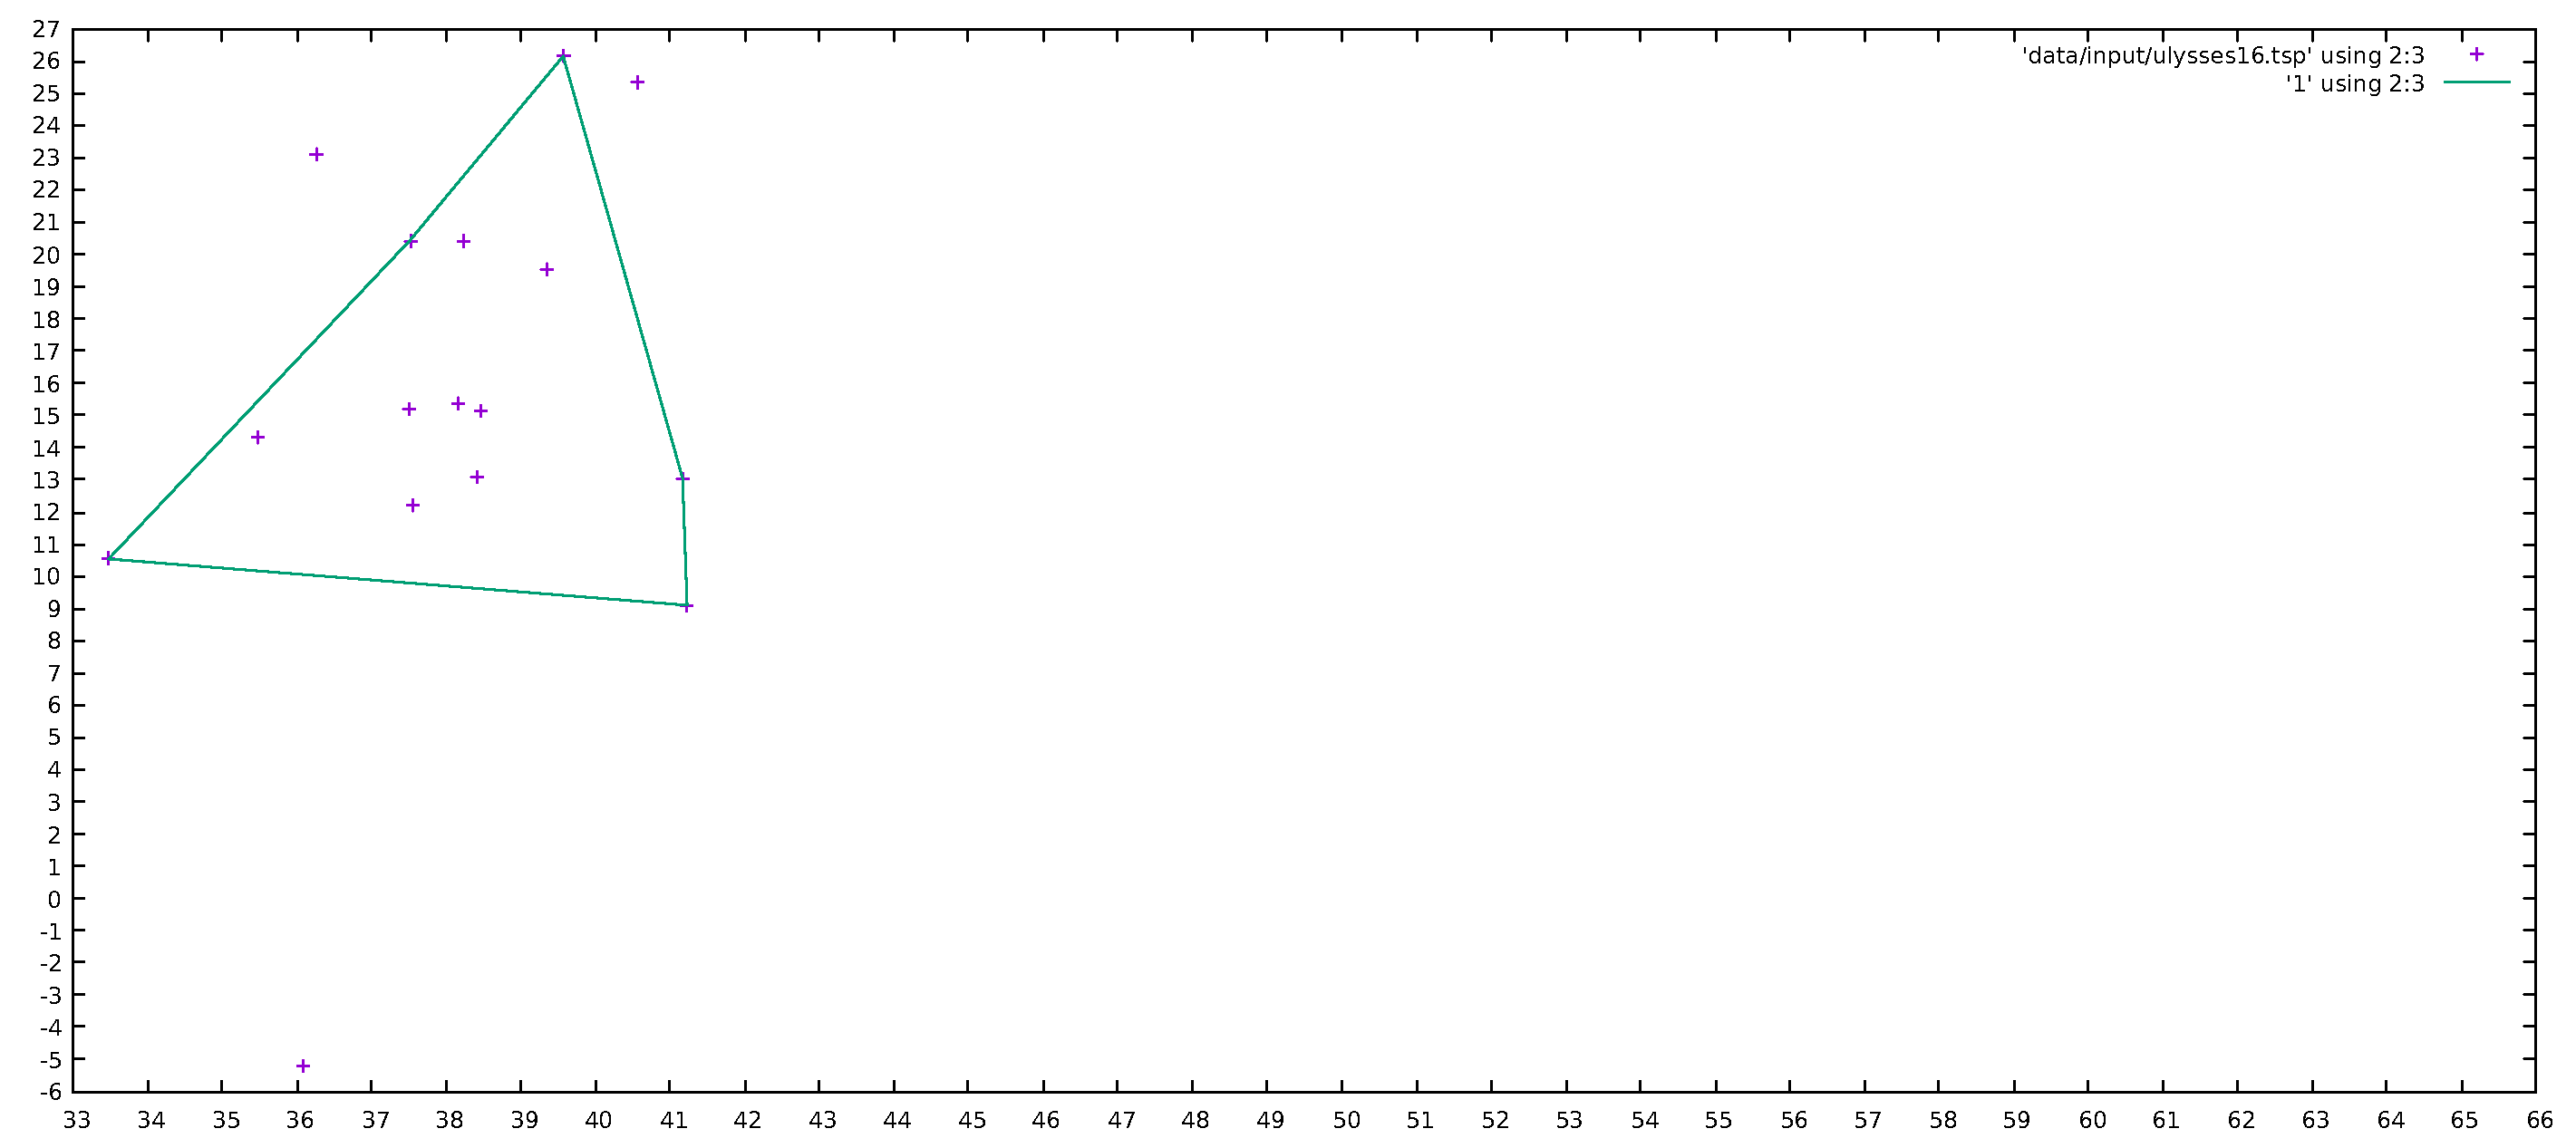
\includegraphics[width=13cm]{data/graphics/insercion/insercion_2.pdf}
\end{figure}
\vspace{0,7cm}

Como podemos comprobar, se añaden las ciudades en el lugar que hagan que el recorrido total sea menor.
\begin{figure}[H]
	\centering
	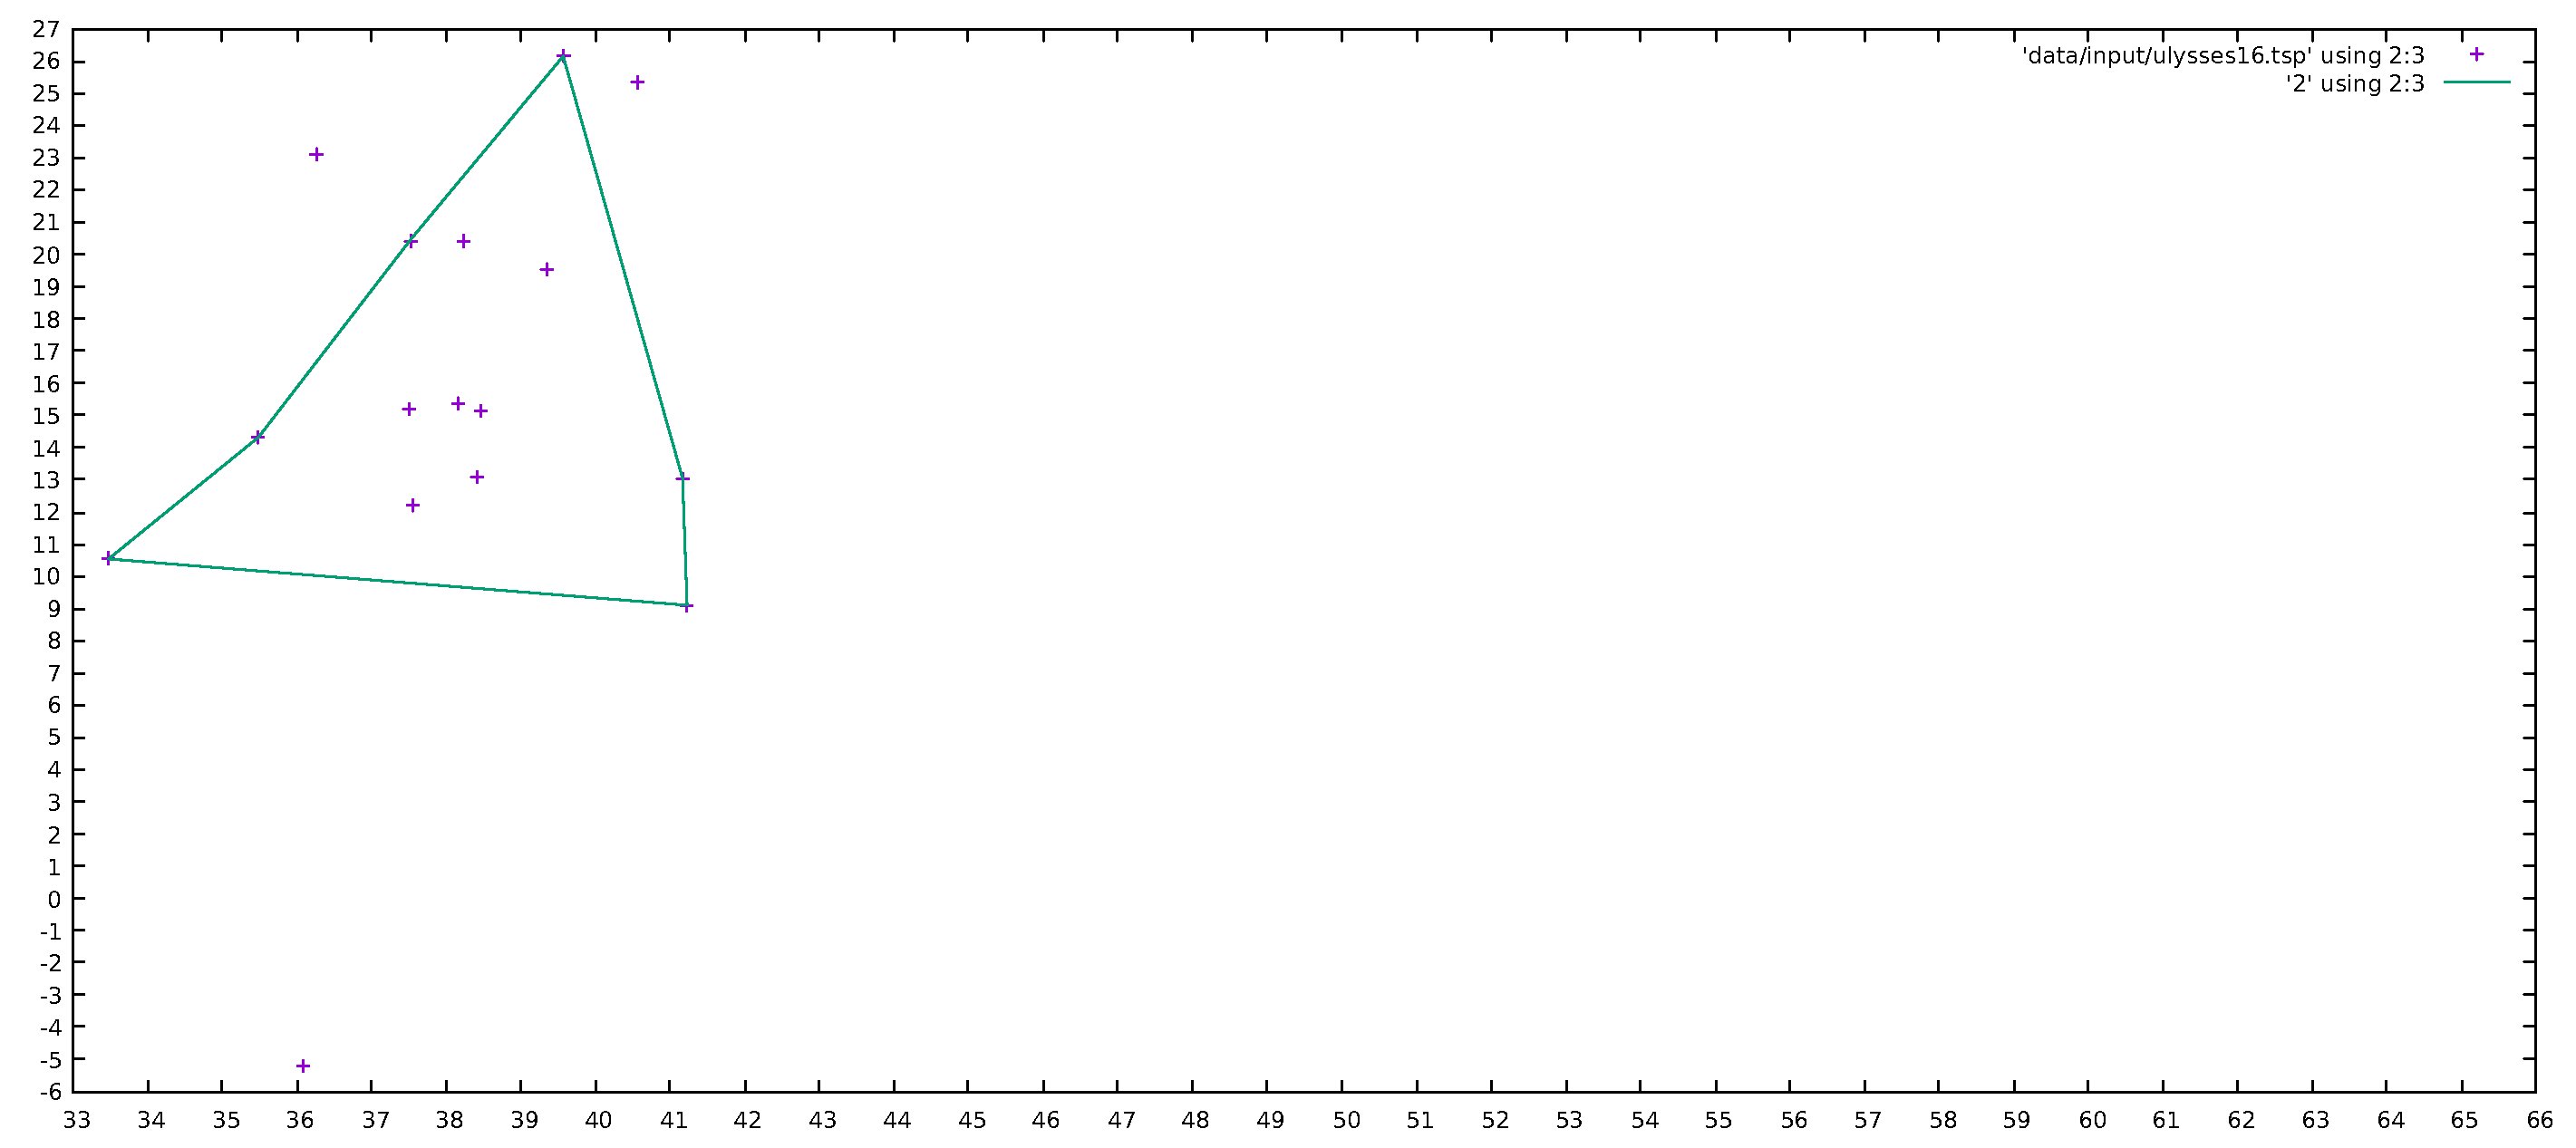
\includegraphics[width=13cm]{data/graphics/insercion/insercion_3.pdf}
\end{figure}
\vspace{0,7cm}

Tras terminar obtenemos el recorrido final.
\begin{figure}[H]
	\centering
	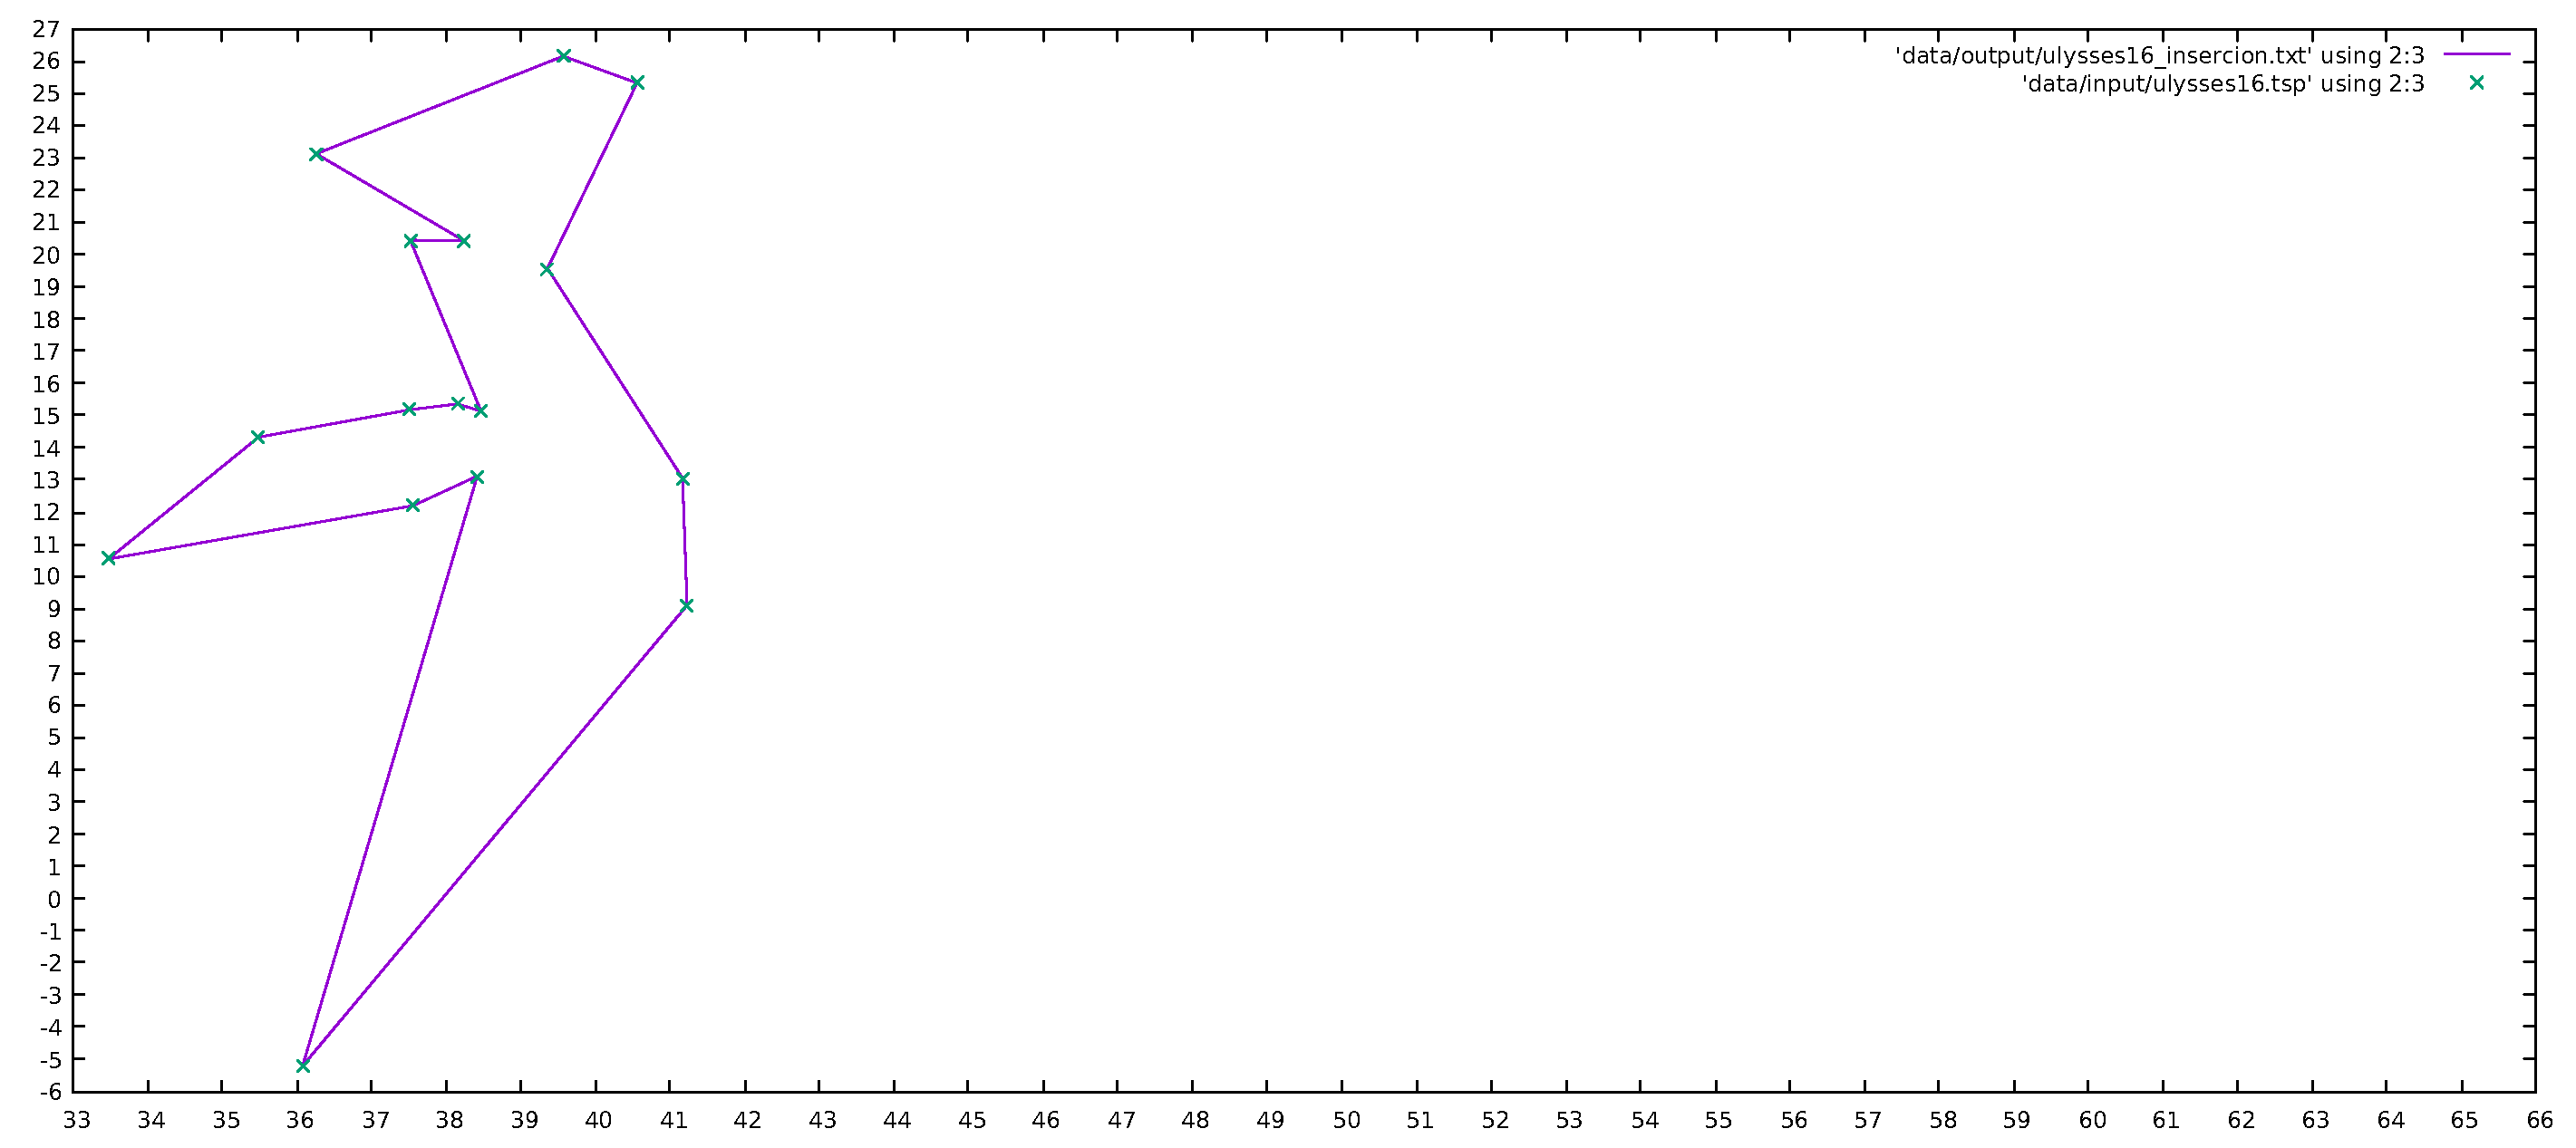
\includegraphics[width=13cm]{data/graphics/insercion/insercion_final.pdf}
\end{figure}

\subsubsection{Eficiencia teórica}
Fijándonos en el pseudocódigo, vemos que la búsqueda de la ciudad del conjunto $V$ que menos aumenta la distancia de $S$ es de orden $O(n^2)$ por lo que estaríamos hablando de un algoritmo de orden $O(n^3)$.


\newpage
\subsection{Algoritmo con otra estrategia}
A continuación, se ha implantado una estrategia nueva para resolver este algoritmo.

\subsubsection{Código del programa}
\begin{lstlisting}[style=C++]
#include <iostream>
#include <fstream>
#include <string>
#include <vector>
#include <utility>
#include <cmath>
#include <limits>
#include <set>
#include "matriz.h"

using namespace std;

double Distancia(const pair<double,double> & posicion_A, const pair<double,double> &posicion_B){
	double distancia = sqrt(pow(posicion_A.first - posicion_B.first,2) + pow(posicion_A.second-posicion_B.second,2));
	
	return distancia;
}

/**
* @brief Estructura que representa una arista del grafo
* @param a Una ciudad del grafo
* @param b Otra ciudad del grafo
* @param distancia Distancia entre la ciudad a y b
*/
struct Arista{
	int a;
	int b;
	double distancia;
};

struct aristaComparator{
	bool operator ()(const Arista arista1, const Arista arista2) const{
		if (arista1.distancia < arista2.distancia)
			return true;
		else 
			return false;
	}
};

/**
* Este programa busca un ciclo que recorra todas las ciudades de 
* un mapa mediante un algoritmo de tipo greedy. En esta version
* del algoritmo, dado un recorrido inicial que contiene tres nodos
* en cada paso se busca el nodo mas cercano al conjunto solucion que
* se encuentre en el conjunto de candidatos. El nodo mas cercano es
* insertado en la posicion del vector que menos aumente el recorrido.
*/
int main(int argc, char **argv){
	const double INF = numeric_limits<double>::max();
	
	if(argc < 2){
		cout << "ERROR. Faltan argumentos [archivo de datos]" << endl;
		exit(-1);
	}
	
	ifstream input_file(argv[1]);
	string line;
	int num_ciudades;
	
	int ciudad;
	double coor_x, coor_y;
	vector<pair<double, double> > v_coordenadas;
	pair<double, double> coordenadas;
	
	vector<int> candidatos;
	vector<int> solucion;
	
	//Movemos el offset a la linea en la que se dice la dimension del grafo
	for(int i=0; i<3; ++i){
		getline(input_file, line);
	}
	
	getline(input_file, line);
	line.erase(0, 11);
	num_ciudades = atoi(line.c_str());
	
	//Reservamos espacio para el grafo
	matriz <double> distancias(num_ciudades, num_ciudades, 0);
	set <Arista, aristaComparator> aristas;
	
	//Movemos el offset al comienzo de los datos
	for(int i=0; i<3; ++i){
		getline(input_file, line);
	}
	
	//Tomamos los datos
	for (int i=0; i<num_ciudades; ++i){
		input_file >> ciudad;
		input_file >> coor_x;
		input_file >> coor_y;
		coordenadas.first = coor_x;
		coordenadas.second = coor_y;
		v_coordenadas.push_back(coordenadas);
	}
	
	//Ordenamos las aristas del grafo de menor a mayor
	for(int i=0; i<num_ciudades; ++i){
		for (int j=i+1; j<num_ciudades; ++j){
			Arista a{i, j, Distancia(v_coordenadas[i], v_coordenadas[j])};
			aristas.insert(a);
		}
	}
	
	//Vector con el grado de cada nodo del grafo solucion
	vector<int> grado(num_ciudades);
	grado.insert(grado.begin(), num_ciudades, 0);
	
	
	
	//Generamos vector de candidatos
	for(int i=0; i<num_ciudades; ++i)
		candidatos.push_back(i);
	
	int tam_solucion = solucion.size(); //Tamanio del conjunto solucion
	
	//Mostramos la solucion
	cout << "Solucion: " << endl;
	
	for(int i=0; i<tam_solucion; ++i){
		cout << solucion[i]+1 << " ";
	}
	cout << endl;
	
	//Calculo de la distancia total recorrida
	double distancia_recorrida = 0.00;
	for(int i=0; i<tam_solucion-1; ++i){
		distancia_recorrida += distancias[i][i+1];
	}
	
	cout << "Distancia total recorrida: " << distancia_recorrida << endl;
	
	//Salida de la solucion a fichero
	ofstream output_file("data/ulysses16_aristas.txt");
	for(int i=0; i<tam_solucion; ++i){
		int c = solucion[i];
		output_file << c+1 << " " << v_coordenadas[c].first << " " << v_coordenadas[c].second << endl;
	}
	
	return (0);
}
\end{lstlisting}

\subsubsection{Pseudocódigo}

\subsubsection{Visualización}

\subsubsection{Eficiencia teórica}


\newpage
\subsection{Comparación de algoritmos}


\newpage
\section{Problema específico}
\subsection{Ahorro de gasolina}
El problema trata de partir de una ciudad y llegar a otra con un vehículo con cierta autonomía pasando por el menor número de gasolineras posibles.\\

Para entender el algoritmo lo podemos imaginar gráficamente. La autonomía del coche va a ser el radio de la circunferencia de centro la primera ciudad o gasolinera en donde nos encontremos en cada momento.\\

Dentro de esa circunferencia se encontrarán las gasolineras a las que podemos llegar con la autonomía del vehículo. Solo nos queda elegir a cual de ellas. Muy facil, nos vamos a la gasolinera que este más cerca de la ciudad objetivo. \\

Así nos vamos moviendo de gasolinera en gasolinera hasta que dentro de nuestra circunferencia se encuentre a la ciudad objetivo.\\

En el desarrollo de este algoritmo nos encontramos un error en tiempo de ejecución de violación de segmento. Esto se debía a que no hacíamos un clear del vector que contenía las distancias desde la posición actual hasta el resto de gasolineras.\\

En el código, más concretamente en la funcion “BuscarGasolinera“,recopilamos las ciudades que están dentro de la circunferencia en el vector de “indices\_posibles\_gasolineras” en donde guardamos los índices de las gasolineras.\\

Después de recopilarlas, buscamos en él, el índice de la gasolinera que minimiza la distancia a la ciudad objetivo y guardamos el índice de aquella que cumple el criterio de optimalidad.\\

La función devuelve el índice que será añadido al vector solución y borrado de manera lógica del vector de candidatos.\\

En el caso de que el índice devuelto de la función sea -1 significa que hemos llegado a un punto en el que desde la gasolinera que nos encontramos no podemos ir a ninguna otra con la autonomía dada. Para indicarlo se muestra un mensaje de error y finaliza el algoritmo.\\

Si el algoritmo finaliza sin mensaje de error significa que se ha conseguido llegar a la ciudad objetivo.\\

\subsubsection{Código del programa}
\begin{lstlisting}[style=C++]
#include <iostream>
#include <fstream>
#include <string>
#include <vector>
#include <utility>
#include <cmath>
#include <limits>
#include "matriz.h"
#include <iomanip>

using namespace std;
const double INF = numeric_limits<double>::max();


double Distancia(const pair<double,double> & posicion_A, const pair<double,double> &posicion_B){

	double distancia = sqrt(pow(posicion_A.first - posicion_B.first,2) + pow(posicion_A.second-posicion_B.second,2));
	
	return distancia;
}

//TODO
int BuscarGasolinera(const int autonomia,const int pos_actual, const int ciudad_destino, matriz<double> & grafo,  vector<int> &candidatos){

	int parada = -1;
	vector<int> indices_posibles_gasolineras;
	double minimo = INF;
	
	for (int i = 0 ;i <candidatos.size();++i){
		double distancia_actual_candidato = grafo[pos_actual][i];
		double distancia_candidato_destino = grafo[i][ciudad_destino];
		if((distancia_actual_candidato <= autonomia) && (candidatos[i] != -1) && (distancia_candidato_destino < minimo)){
			parada = i;
			minimo = distancia_candidato_destino;
		}
	}
	
	return(parada);
}

int main(int argc, char **argv){

	string line;
	int num_ciudades;
	
	if(argc<5){
		cout << "Faltan argumentos:\n" "./gasolineras [archivo] [autonomia] [ciudad origen] [ciudad destino]" << endl;
	}
	
	ifstream input_file(argv[1]);
	double autonomia = atoi(argv[2]);
	int ciudad_origen = atoi(argv[3]) - 1;
	int ciudad_destino = atoi(argv[4]) - 1;
	int pos_actual = ciudad_origen;
	
	//Variables que usaremos para crear la matriz de distancias (grafo)
	int ciudad;
	double coor_x, coor_y;
	vector<pair<double, double> > v_coordenadas;
	pair<double, double> p;
	
	//Movemos el offset a la linea en la que se dice la dimension del grafo
	for(int i=0; i<3; ++i){
		getline(input_file, line);
	}
	
	getline(input_file, line);
	line.erase(0, 11);
	num_ciudades = atoi(line.c_str());
	
	//Reservamos espacio para el grafo
	matriz<double> distancias(num_ciudades, num_ciudades, 0);
	
	
	//Movemos el offset al comienzo de los datos
	for(int i=0; i<3; ++i){
		getline(input_file, line);
	}
	
	//Tomamos los datos
	for (int i=0; i<num_ciudades; ++i){
		input_file >> ciudad;
		input_file >> coor_x;
		input_file >> coor_y;
		p.first = coor_x;
		p.second = coor_y;
		v_coordenadas.push_back(p);
	}
	
	//Calculamos las distancias y las metemos en la matriz que representa
	//el grafo
	for(int i=0; i<num_ciudades; ++i){
		for (int j=i+1; j<num_ciudades; ++j){
			distancias[i][j]=Distancia(v_coordenadas[i], v_coordenadas[j]);
			distancias[j][i]=distancias[i][j];
		}
	}
	
	//Comienzo del algoritmo
	vector<int> candidatos;
	vector<int> solucion;
	solucion.push_back(ciudad_origen);
	
	for(int i = 0; i< num_ciudades; i++)
		candidatos.push_back(i);
	
	candidatos[ciudad_origen] = -1;
	bool fin = false;
	pos_actual = ciudad_origen;
	
	
	while(fin == false){
		if(autonomia >= distancias[pos_actual][ciudad_destino]){
			cout << "FIN = DESTINO" <<  endl;
			solucion.push_back(ciudad_destino);
			fin = true;
		}
	
		else{
			pos_actual = BuscarGasolinera(autonomia,pos_actual, ciudad_destino, distancias, candidatos);
		
			if(pos_actual != -1){
				candidatos[pos_actual] = -1;
				solucion.push_back(pos_actual);
			}
			else{
				cout << "No podemos llegar a ninguna otra gasolinera" << endl;
				fin = true;
			}
		}
	}
	
	for (int i = 0; i<solucion.size(); ++i){
		cout << solucion[i]+1 << " --> ";
	}
	
	cout << "FIN" << endl;
	
	ofstream ficherosalida("data/gasolineras.txt");
	for (int i = 0; i < solucion.size(); ++i){
		int c = solucion[i];
		ficherosalida << c+1 << " " << v_coordenadas[c].first << " " << v_coordenadas[c].second << endl;
	}
	
	return(0);
}
\end{lstlisting}

\subsubsection{Pseudocódigo}
\begin{lstlisting}
Mientras no se llegue al destino o a un punto sin salida:
	Encontrar gasolineras / ciudades posibles con la autonomia;
	Si podemos ir a gasolineras o a la ciudad objetivo:
		Si podemos ir a la ciudad objetivo:
			FIN;
		Si podemos ir a una o varias gasolineras:
			Elegir la mas cercana a la ciudad objetivo;
			Anadir al vector solucion;
			Posicionarnos en la nueva gasolinera;
	Si no podemir a ningun lado:
		FIN;
\end{lstlisting}



\subsubsection{Visualización}
\begin{figure}[H]
	\centering
	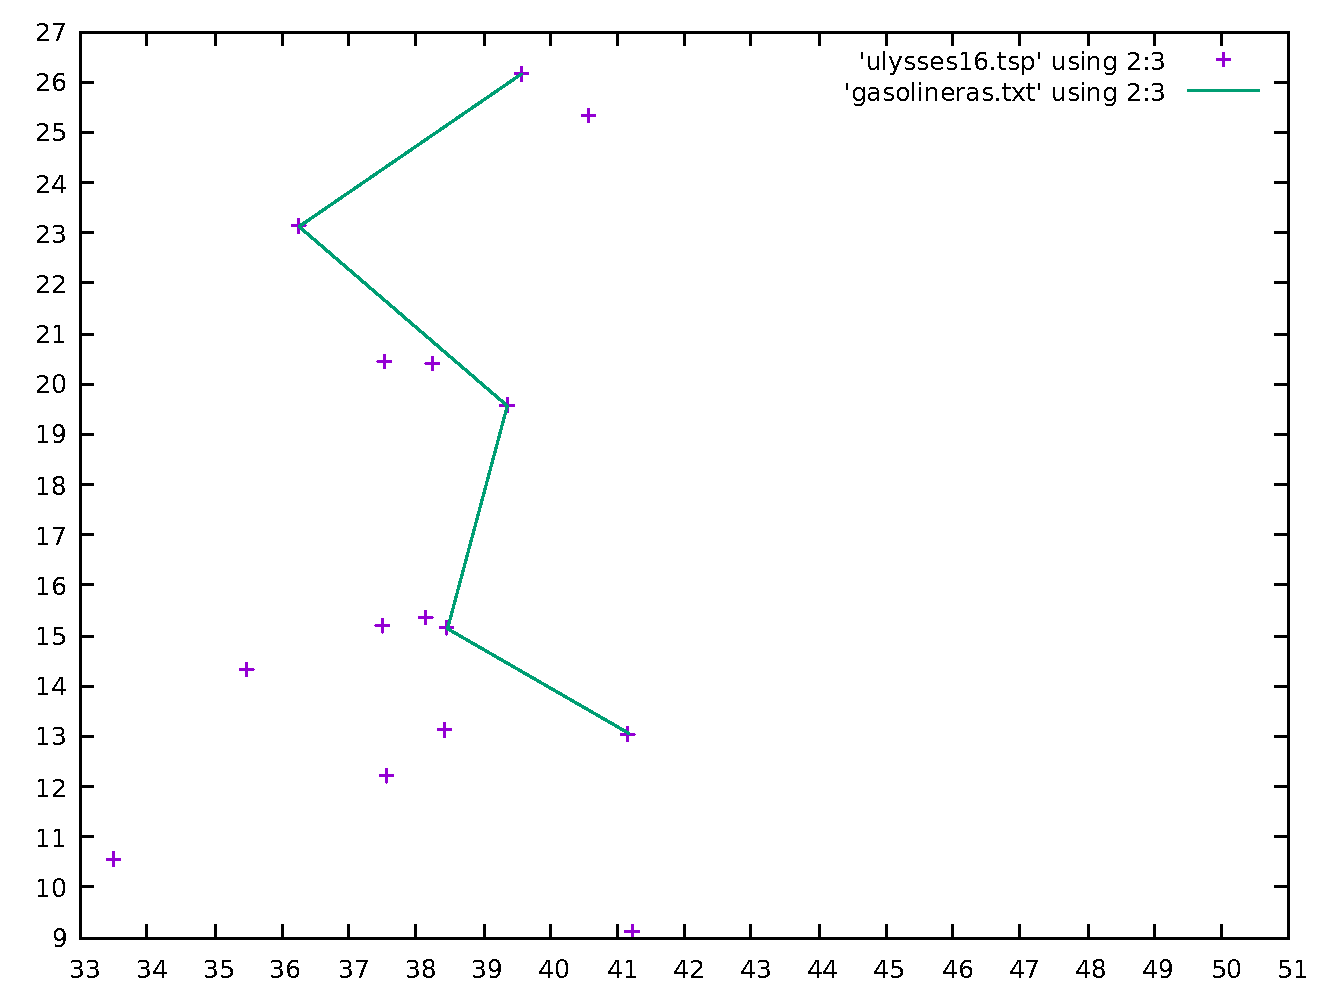
\includegraphics[width=13cm]{data/graphics/gasolineras/gasolineras.pdf}
\end{figure}

\subsubsection{Eficiencia teórica}
La eficiencia teórica O(n) depende del número de ciudades que hay. Tomamos, por tanto, $TAM = num\_ciudades = n$.\\

La eficiencia del algoritmo, en el peor de los casos, es 
$$T(n) = \sum_{i=1}^{n}\sum_{j=i}^{n}$$
$$T(n) = n*(n-i)$$
$$T(n) \in O(n^2)$$\\

Para hallar esto nos debemos de fijar en el bucle que comienza en la línea 112 y analizarlo. Nos damos cuenta que, en el peor de los casos, el algoritmo revisa todas las ciudades y escoge la última, y luego vuelve a revisarlas todas y escoger la última, y así consecutivamente.


%----------------------------------------------------------------------------------------

%\marginnote{\textbf{NOTA}: Algoritmo al que calcular la eficiencia.}

\end{document}